\documentclass[A4, twocolumn]{article}
\usepackage{ucs}
\usepackage[T1,T2A]{fontenc}
\usepackage[utf8x]{inputenc}
\usepackage[english]{babel}  
\usepackage{amsmath}
\usepackage{amssymb}
\usepackage{mathtools}
\usepackage{hyperref}
\usepackage{graphicx}
\usepackage{caption}
\usepackage{xcolor}
\usepackage{hyperref}
\usepackage{ dsfont }
\usepackage{graphicx}

\usepackage{titlesec} % Allows customization of titles
\renewcommand\thesection{\Roman{section}} % Roman numerals for the sections
\renewcommand\thesubsection{\roman{subsection}} % roman numerals for subsections
\titleformat{\section}[block]{\large\scshape\centering}{\thesection.}{1em}{} % Change the look of the section titles
\titleformat{\subsection}[block]{\large}{\thesubsection.}{1em}{} % Change the look of the section titles


% Цвета для гиперссылок
\definecolor{linkcolor}{HTML}{00008B} % цвет ссылок
\definecolor{urlcolor}{HTML}{00008B} % цвет гиперссылок
 
\hypersetup{pdfstartview=FitH,  linkcolor=linkcolor,urlcolor=urlcolor, colorlinks=true}

\graphicspath{{pictures/}}

\DeclareGraphicsExtensions{.pdf,.png,.jpg}

\newtheorem{Def}{Definition}

\newtheorem{Fact}{Fact}

\newtheorem{Th}{Theorem}

\newtheorem{Lem}{Lemm}

\newenvironment{PROOF}
{\par\noindent{\bf Доказательство:}\newline$\triangleright$}
{\hfill$\scriptstyle\blacktriangleleft$}

\usepackage[left=2cm,right=2cm,top=2cm,bottom=2cm,bindingoffset=0cm]{geometry}

\title{
\textbf{An Introduction to Differential Evolution} 
}

\date{\today}
\author{ 
	\textsc{Mikhaylov Nikita, Polyanski Maxim} \\
	\normalsize \href{mailto:mikhaylovnikitka@phystech.edu}{mikhaylovnikitka@phystech.edu} \\
	\normalsize \href{mailto:polyanskiy.mn@phystech.edu}{polyanskiy.mn@phystech.edu} \\
	\normalsize \href{https://github.com/nikitamikhaylov/differential-evolution}{https://github.com/nikitamikhaylov/differential-evolution}
}

\usepackage{titling}
\renewcommand{\maketitlehookd}{
	It is a brief description of one of the most famous genetic algorithms of real optimization - the algorithm of differential evolution (Differential Evolution, DE). For complex problems of optimizing the function of n variables, this algorithm has such good properties that it can often be considered as a ready-made “building block” when solving many problems of identification and pattern recognition. For example it is used in "One pixel attack for fooling deep neural networks" problem.
}

\begin{document}

    \maketitle
    
	%----------------------------------------------------------
	
  \section{\textbf{Why use Differential Evolution?}}	
	\begin{itemize}
		\item Global optimisation is necessary in fields such as engineering, statistics
		and finance
		
		\item But many practical problems have objective functions that are nondifferentiable,
		non-continuous, non-linear, noisy, flat, multi-dimensional
		or have many local minima, constraints or stochasticity
		
		\item Such problems are difficult if not impossible to solve analytically
		
		\item DE can be used to find approximate solutions to such problems
	\end{itemize}		
	
	
	\section{\textbf{The Basics of Differential Evolution}}
	
		\begin{itemize}
			\item Stochastic, population-based optimisation algorithm.
			\item Introduced by Storn and Price in 1996.
			\item Developed to optimise real parameter, real valued functions. 
			\item General problem formulation is: 
			
			 For an objective function $f : X \subseteq \mathds{R}^D \rightarrow  \mathds{R}$ where the feasible region $X \neq \varnothing$, the minimisation problem is to find:
			 
			 $x^{∗} \in X$ such that $f(x^{∗}) \leq f(x) \forall x ∈ X $  \\ where: \\ $f(x^{∗}) \neq − \infty $
		\end{itemize}
	%---------------------------------------------------------
	
	\section{\textbf{Basic Algorithm}}
	DE is an Evolutionary Algorithm. This class also includes Genetic Algorithms, Evolutionary Strategies and
	Evolutionary Programming. 
	
	
	\begin{figure}
		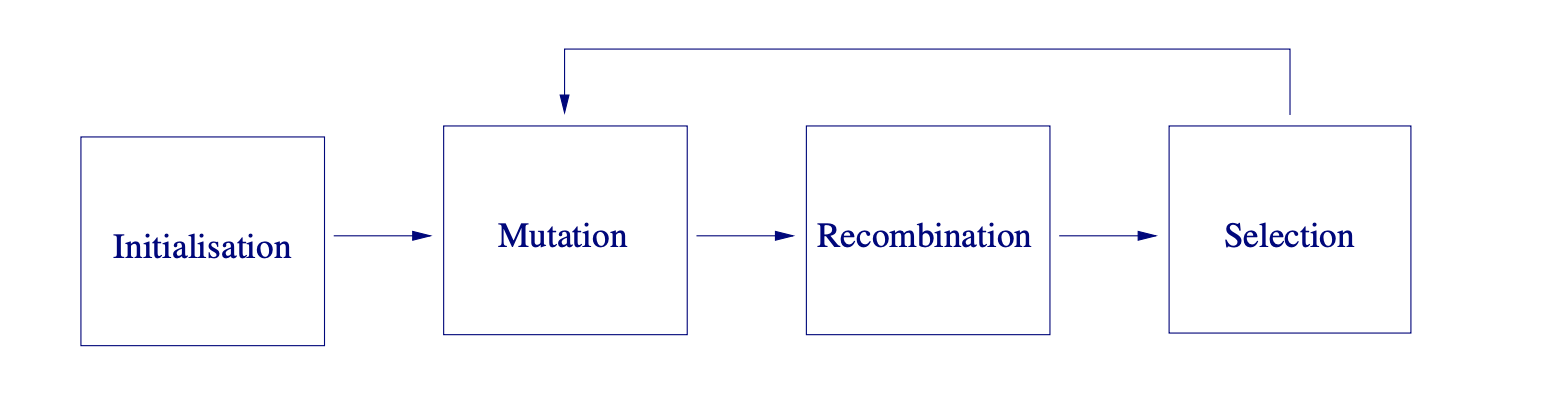
\includegraphics[width=\linewidth]{schema.png}
		\caption{General Evolutionary Algorithm Procedure}
		\label{fig:General Evolutionary Algorithm Procedure}
	\end{figure}

	
	
	\begin{itemize}
		\item{\textbf{Notation}}
		
		Suppose we want to optimise a function with D real parameters. We must select the size of the population N (it must be at least 4). The parameter vectors have the form:
		
		$x_{i, G} = [x_{1, i, G}, x_{2,i,G}, ..., x_{D,i,G}], i = 1, 2, ..., N$
		
		where G is the generation number.
		
		\item{\textbf{Initialisation}}
		
		Define upper and lower bounds for each parameter:
		
		$ x^{L}_{j} \leq x_{j,i,1} \leq x^{U}_{j}$
		
		Randomly select the initial parameter values uniformly on the intervals $[x^{L}_{j}, x^{U}_{j}]$
		\item{\textbf{Mutation}}
		
		Each of the N parameter vectors undergoes mutation, recombination and
		selection. Mutation expands the search space. For a given parameter vector $x_{i, G}$ randomly select three vectors $x_{r1, G}$, $x_{r2, G}$ and $x_{r3, G}$ such that the indices $i$, $r1$, $r2$ and $r3$ are distinct. Then add the weighted difference of two of the vectors to the third. 
		$v_{i, G+1} = x_{r1, G} + F(x_{r2, G} - x_{r3, G})$		
		
		The  mutation factor $F$ is a constant from [0, 2] and $v_{i, G+1}$ is called the donor vector. 
		\item{\textbf{Recombination}}
		
		Recombination incorporates successful solutions from the previous generation. The trial vector $u_{i,G+1}$ is developed from the elements of the target vector, $x_{i,G}$, and the elements of the donor vector, $v_{i,G+1}$. Elements of the donor vector enter the trial vector with probability CR. 
		
	
		\[
		u_{j,i,G+1} = \left\{
		\begin{array}{lr}
		v_{j,i,G+1}, & \text{if } rand_{j,i} \leq CR \\
		& \text{ or } j = I_{rand}\\
		x_{j,i,G}, & \text{otherwise }
		\end{array} \right\}
		\]
		
		$i = 1,2,...,N$
		$j = 1,2,...,D$ \\
		$rand_{j,i} ∼ U[0, 1]$, $I_{rand}$ is a random integer from $[1, 2, ..., D]$
		and $I_{rand}$ ensures that $v_{i,G+1} \neq x_{i,G}$
		
		\item{\textbf{Selection}}
		
		The target vector $x_{i,G}$ is compared with the trial vector $v_{i,G+1}$ and the
		one with the lowest function value is admitted to the next generation
		
		
		\[
		u_{i,G+1} = \left\{
		\begin{array}{lr}
		u_{i,G+1}, & \text{if } f(u_{i,G+1}) \leq f(x_{i, G})\\
		x_{i,G}, & \text{otherwise }
		\end{array} \right\}
		\]
		
		Mutation, recombination and selection continue until some stopping criterion
		is reached.
	\end{itemize}

	\section{\textbf{Examples}}
	
	The functions listed below are some of the common functions used for testing optimization algorithms.
	
	\subsection*{\textbf{Ackley Function}}
	
	$f(\textbf{x}) = f(x_1, ..., x_n) =\\
	 -a \exp(-b\sqrt{\frac{1}{n}\sum_{i=1}^{n}x_i^2})-exp(\frac{1}{n}\sum_{i=1}^{n}cos(cx_i))+ a + e$ \\
	 
	 In the above equation, the values $a, b, c$ are constants and are usually 
	 chosen as $a = 20$, $b = 0.2$ and $c = 2\pi$ \\
	 
	 This function is continuous, not convex, defined on n-dimensional space, multimodal (Figure 2.). The Ackley function can be defined on any input domain but it is usually evaluated on $x \in [-32, 32]$ for all $i = 1, ..., n$. It has one global minimum at: $f(x^*) = 0$ at $x^* = (0, ..., 0)$. 
	 
	 Figure 3. shows the Ackley Funciton's convergence with mutation factor $F = 0.7$ and $rand_{ji} = 0.9$. On Figure 4. there are DE's outputs with different hyperparameters which are found with grid. The $rand_{ji}$ is horizontal axis and mutation factor is vertical axis.
	 \begin{figure}
	 	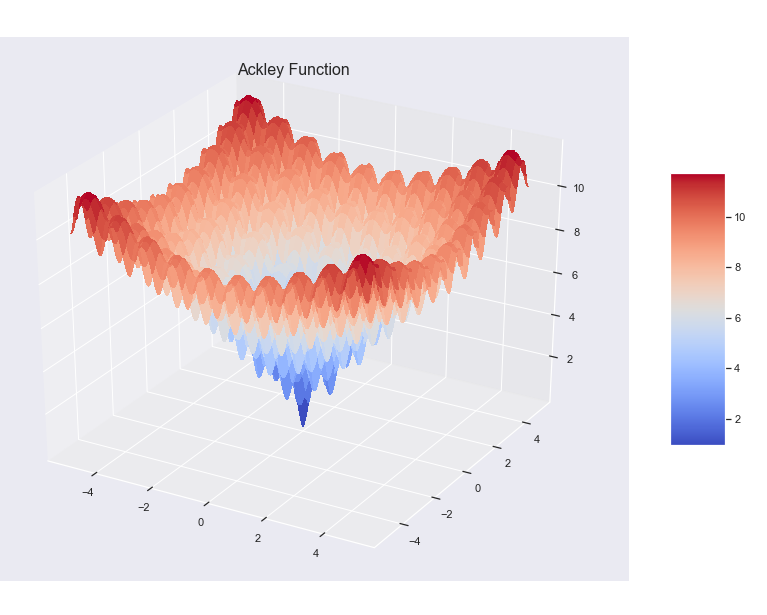
\includegraphics[width=\linewidth]{ackley/ackley_plot.png}
	 	\caption{Ackley Function Plot}
	 	\label{fig:Ackley Function Plot}
	 \end{figure}
 
  
	 \begin{figure}
	 	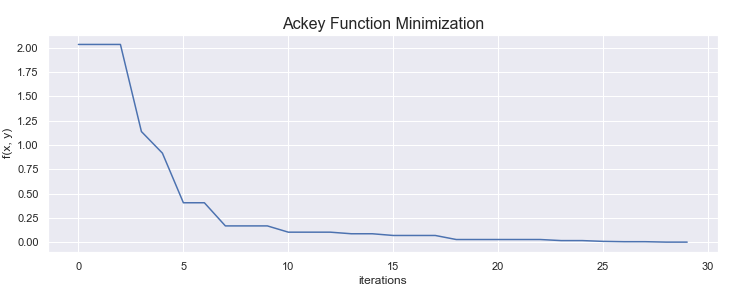
\includegraphics[width=\linewidth]{ackley/ackley_convergence.png}
	 	\caption{Ackley Function Convergence}
	 	\label{fig:Ackley Function Convergence}
	 \end{figure}
 
	  \begin{figure}
	 	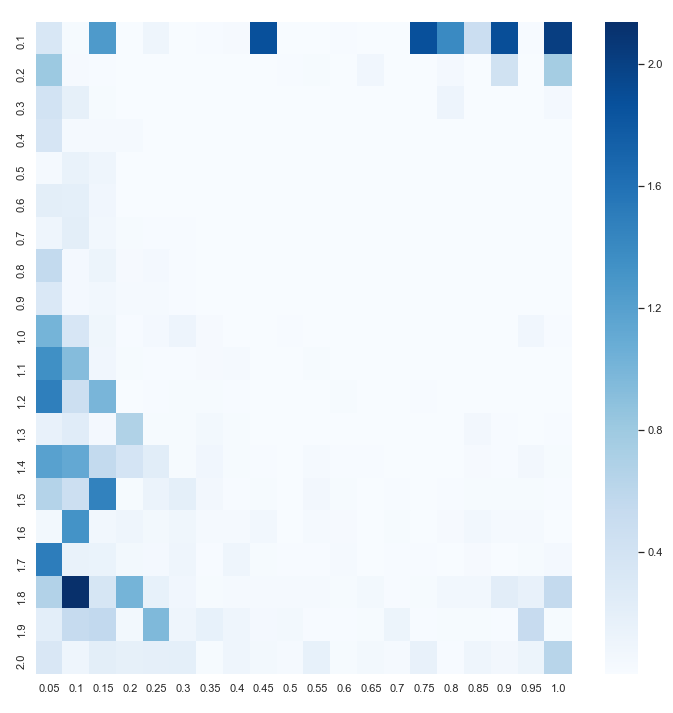
\includegraphics[width=\linewidth]{ackley/ackley_heatmap.png}
	 	\caption{Ackley Function Heatmap}
	 	\label{fig:Ackley Function Heatmap}
	 \end{figure}

 
 	\subsection*{\textbf{Bartels Conn Function}}
 	
 	$f(x,y)=|x^2 + y^2 + xy| + |sin(x)| + |cos(y)|$
 	
 	This function is not convex, defined on 2-dimensional space, non-separable, non-differentiable. It can be defined on any input domain but it is usually evaluated on $x \in [-500, 500]$ and $y \in [-500, 500]$. The global minimum $f(x^*) = 1$ is located at $x^* = (0,0)$.
 	
 	Figure 6. shows the Bartes Conn's convergence with mutation factor $F = 0.7$ and $rand_{ji} = 0.9$. After 20 iterations the global optimum was found. On Figure 7. there are DE's outputs with different hyperparameters which are found with grid. The $rand_{ji}$ is horizontal axis and mutation factor is vertical axis.
 	
 	\begin{figure}
 		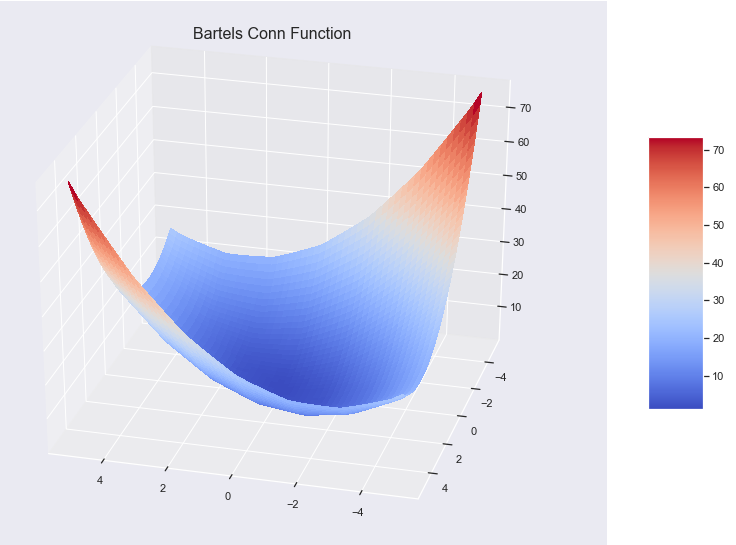
\includegraphics[width=\linewidth]{bartels_conn/bartels_conn_plot.png}
 		\caption{Bartels Conn Function Plot}
 		\label{fig:Bartels Conn Function Plot}
 	\end{figure}
 	
 	
 	\begin{figure}
 		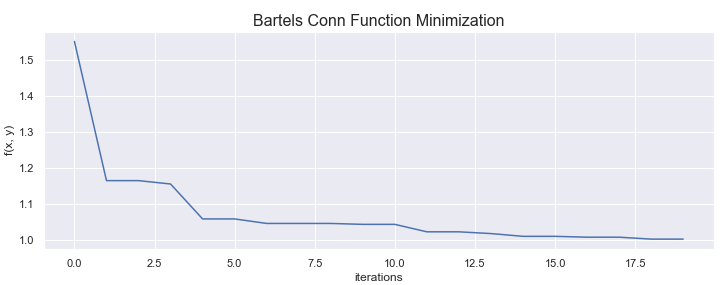
\includegraphics[width=\linewidth]{bartels_conn/bartels_conn_convergence.png}
 		\caption{Bartels Conn Function Convergence}
 		\label{fig:Bartels Conn Function Convergence}
 	\end{figure}
 	
 	\begin{figure}
 		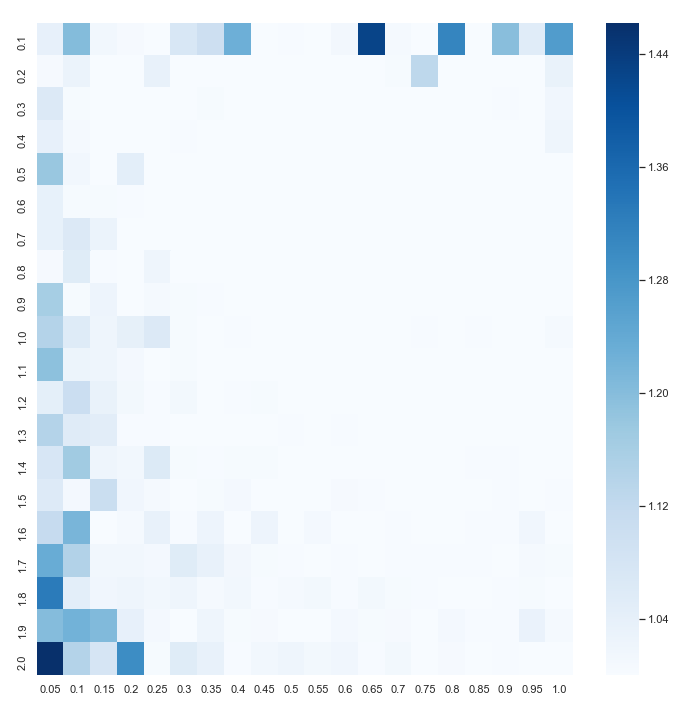
\includegraphics[width=\linewidth]{bartels_conn/bartels_conn_heatmap.png}
 		\caption{Bartels Conn Function Heatmap}
 		\label{fig:Bartels Conn Function Heatmap}
 	\end{figure}
 
 
	 \subsection*{\textbf{Xin-She Yang Function}}
	 
	 $f(\mathbf x)=f(x_1, ...,x_n)=\sum_{i=1}^{n}\epsilon_i|x_i|^i$ \\
	 
	 Where $\epsilon$ is a random number that is drawn uniformly from $[0, 1]$
	 
	 This function is not convex, defined on n-dimensional space, separable, non-differentiable. The Xin-She Yang Function can be defined on any input domain but it is usually evaluated on $x \in [-5, 5]$ for all $i = 1,...,n$. It has one global minimum at: $f(x^*) = 0$ at $x^* = (0, ..., 0)$. Figure 9. shows the Bartes Conn's convergence with mutation factor $F = 0.7$ and $rand_{ji} = 0.9$. After about 20 iterations the global optimum was found. On Figure 10. there are DE's outputs with different hyperparameters which are found with grid. The $rand_{ji}$ is horizontal axis and mutation factor is vertical axis.
	 
	 In addition, it is recommended to use $F \in [0.4, 1]$ to get better results. Heatmaps also prove this statement.
	
	 \begin{figure}
	 	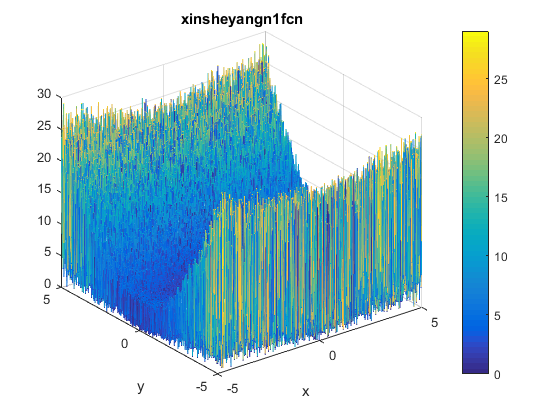
\includegraphics[width=\linewidth]{xin_she_yang/xin_she_yang_plot.png}
	 	\caption{Xin-She Yang Function Plot}
	 	\label{fig:Xin-She Yang Function Plot}
	 \end{figure}
	 
	 
	 \begin{figure}
	 	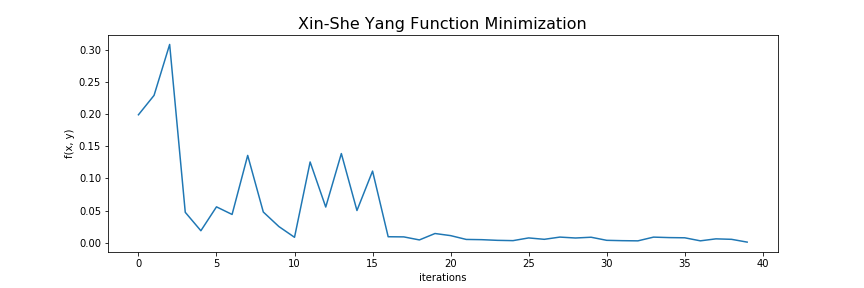
\includegraphics[width=\linewidth]{xin_she_yang/xin_she_yang_convergence.png}
	 	\caption{Xin-She Yang Function Convergence}
	 	\label{fig:Xin-She Yang Function Convergence}
	 \end{figure}
	 
	 \begin{figure}
	 	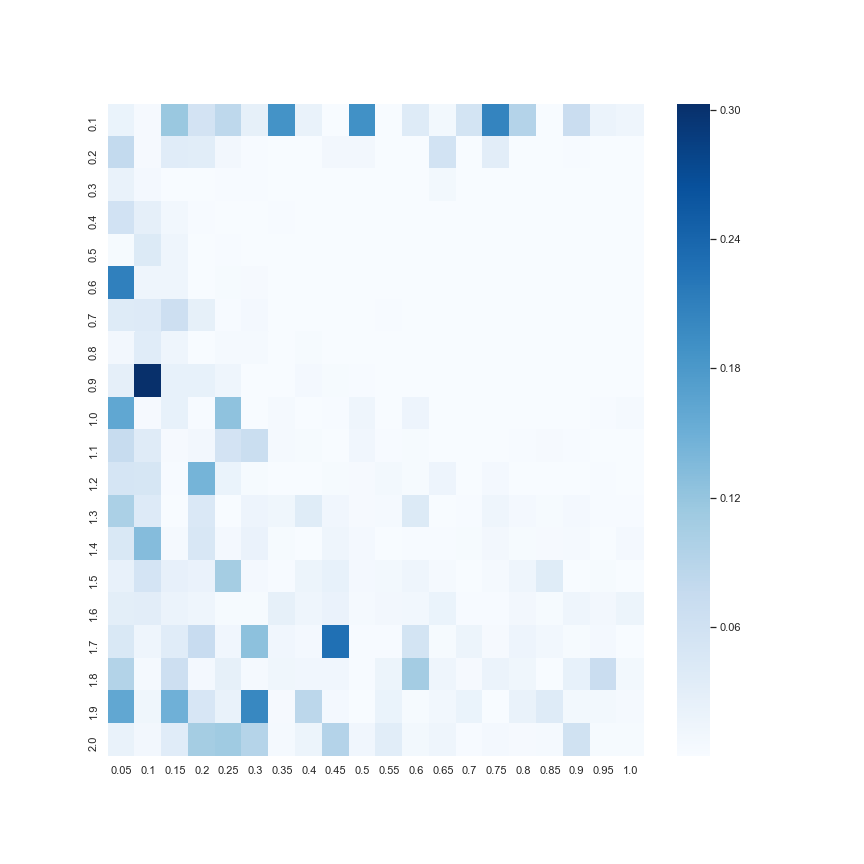
\includegraphics[width=\linewidth]{xin_she_yang/xin_she_yang_heatmap.png}
	 	\caption{Xin-She Yang Function Heatmap}
	 	\label{fig:Xin-She Yang Function Heatmap}
	 \end{figure}
 
	
	\section{\textbf{Performance}}
	
	\begin{itemize}
		\item There is no proof of convergence for DE
		\item However it has been shown to be effective on a large range of classic
		optimisation problems
		\item In a comparison by Storn and Price in 1997 DE was more efficient than
		simulated annealing and genetic algorithms
		\item Ali and Torn (2004) found that DE was both more accurate and more
		efficient than controlled random search and another genetic algorithm
		\item In 2004 Lampinen and Storn demonstrated that DE was more accurate
		than several other optimisation methods including four genetic algorithms,
		simulated annealing and evolutionary programming
	\end{itemize}


	\section{\textbf{Recent Applications}}
	
	\begin{itemize}
		\item Design of digital filters
		\item Optimisation of strategies for checkers
		\item Maximisation of profit in a model of a beef property
		\item Optimisation of fermentation of alcohol
	\end{itemize}

	%----------------------------------------------------------
	
	
	\section{\textbf{References}}
	\begin{enumerate}
		
		\item Differential Evolution:A Practical Approach to Global Optimization, Price, Kenneth, Storn, Rainer M., Lampinen, Jouni A.
		
		\item Differential Evolution: In Search of Solution, Feoktistov, Vitaliy
		
		\item Price, K.V. (1999), ‘An Introduction to Differential Evolution’ in Corne,
		D., Dorigo, M. and Glover, F. (eds), New Ideas in Optimization, McGrawHill,
		London
		
		\item Storn, R. and Price, K. (1997), ‘Differential Evolution - A Simple and Efficient
		Heuristic for Global Optimization over Continuous Spaces’, Journal
		of Global Optimization, 11, pp. 341–359.
		
		\item \href{http://www.sfu.ca/~ssurjano/ackley.html}{http://www.sfu.ca/~ssurjano/ackley.html}
		
		\item \href{https://en.wikipedia.org/wiki/Test_functions_for_optimization}{https://en.wikipedia.org/wiki/Test-functions-for-optimization}

		
		\item Momin Jamil and Xin-She Yang, A literature survey of benchmark functions for global optimization problems, Int. Journal of Mathematical Modelling and Numerical Optimisation, Vol. 4, No. 2, pp. 150–194 (2013), arXiv:1308.4008
		
		\item Momin Jamil and Xin-She Yang, A literature survey of benchmark functions for global optimization problems, Int. Journal of Mathematical Modelling and Numerical Optimisation, Vol. 4, No. 2, pp. 150–194 (2013), arXiv:1308.4008
	
		\item X. S. Yang, “Test Problems in Optimization,” Engineering Optimization: An Introduction with Metaheuristic Applications John Wliey  Sons, 2010. [Available Online]: http://arxiv.org/abs/1008.0549
	\end{enumerate}
	 	
	%----------------------------------------------------------
	 
	 
   
\end{document}